\subsection*{Design}
In \myref{subsec:Scope} the scope of identifiers, variables and functions, are defined for \gls{gamble}.
A variable is in scope from its declaration until the end of the block it is declared in.
An inner scope inherits the identifiers declared in the outer scopes. 

During contextual analysis it is important to verify that each variable and function used are in scope and if not it should produce a descriptive error message.
The error message should indicate which identifier is not in scope, and the line this identifier is introduced on.

To check this all references to identifiers must be checked to see if they match an identifier in the symbol table of the current scope, and recursively the scope which encloses it. 
Furthermore it is important that any usage of an identifier only exists after its declaration.
In the compiler for \gls{gamble}, the symbol table is filled while the compiler is also performing the scope checking.
This is because it reduces the amount of traversals through the tree, scope checking and filling the symbol table is also of similar concept, e.g. a declaration creates an entry in the symbol table, while expressions simply use lookups in this table.

The scope checker can produce two types of errors: redeclaration errors and undeclared errors.
A redeclaration error is produced when attempting to declare a variable, while one with the same name is already declared in scope.
An undeclared error is produced when an attempt to use a variable which is not declared in the current scope or any enclosing scopes are made. 
Examples are shown in \myref{lst:scopeErrors}.

\begin{lstlisting}[caption=Examples of scope errors in \gls{gamble}, numbers=none,frame=tlrb,label={lst:scopeErrors}]
// [...]
int a = 1;
float a = 2.2;   // Redeclaration error
int a = 2;       // Redeclaration error 

b = 2;           // Undeclared error   
int b = 0;
b = foo();       // Redeclaration error and undeclared error 
// [...]
\end{lstlisting}

The design of the classes involved in the Scopechecking subphase can be seen on \myref{fig:scopeCheck}.

\begin{figure}
\centering
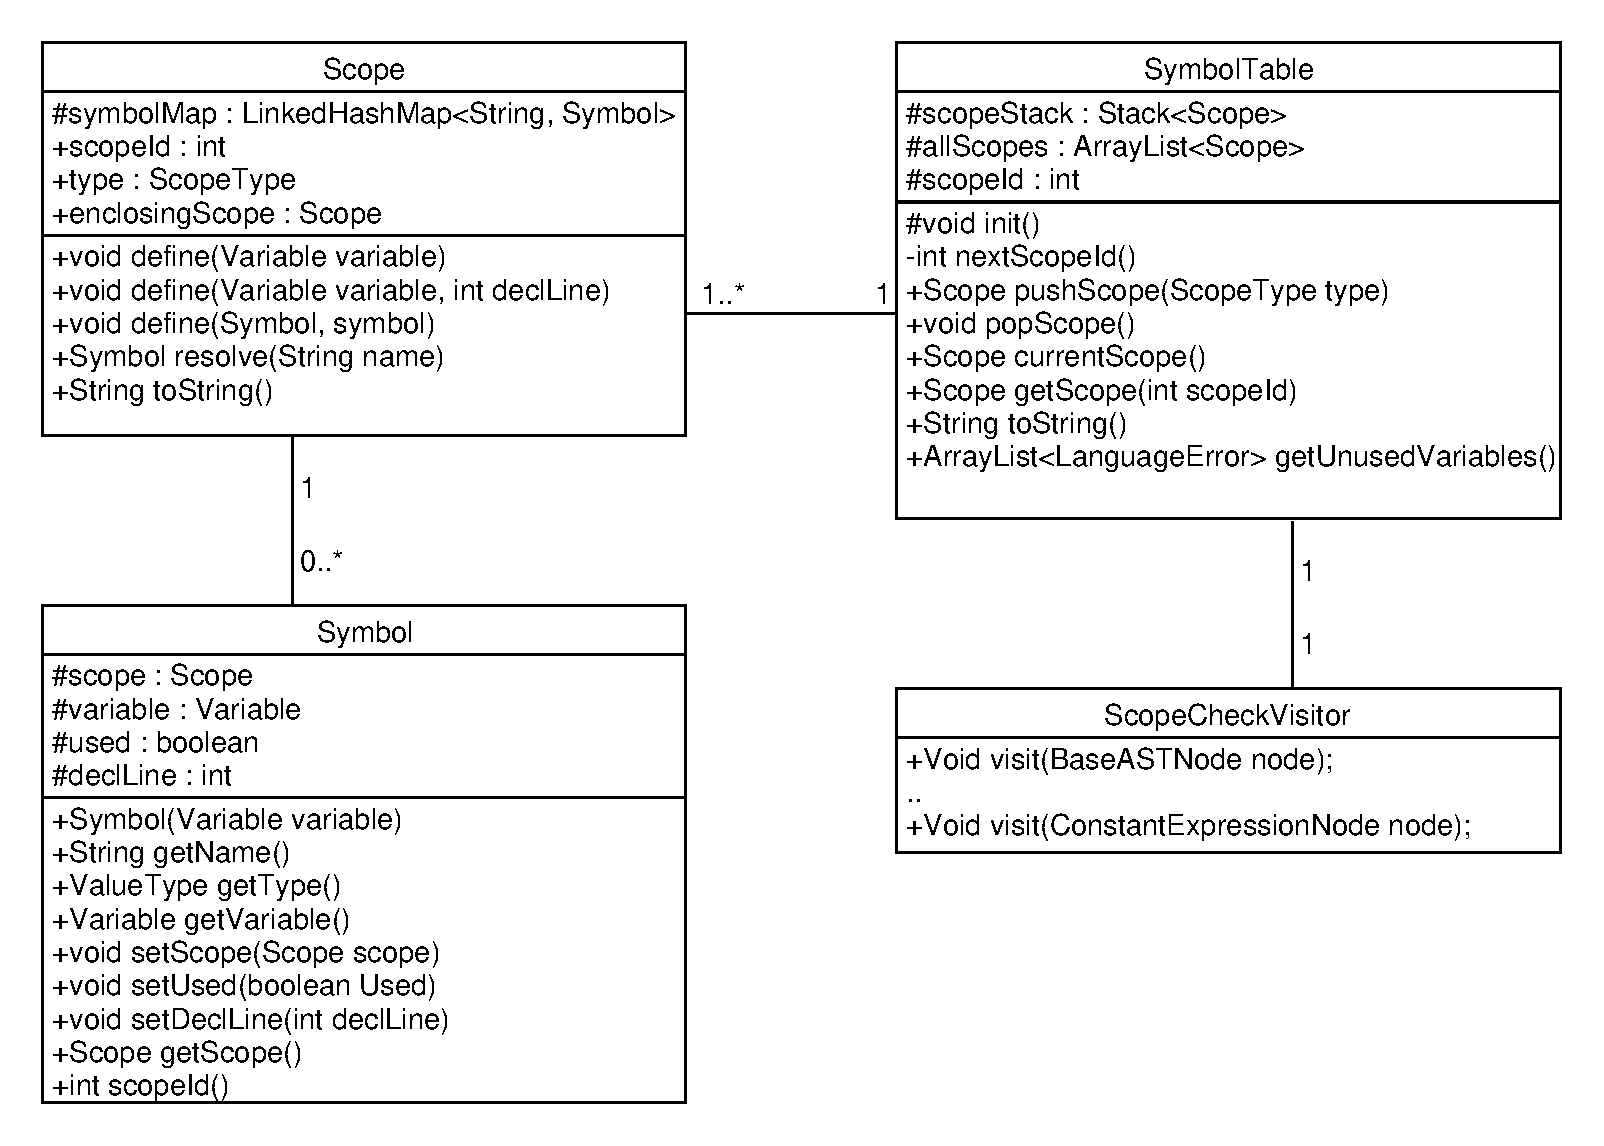
\includegraphics[width=1\textwidth]{figures/ClassDiagrams/ScopeCheck.pdf}
\caption{Class diagram showing the different classes involved in scope checking and their associations.}
\label{fig:scopeCheck}
\end{figure}
\vspace{-15pt}

\subsection*{Implementation}
In the \gls{gamble} compiler, the class \texttt{SymbolTable} represents a collection of scopes.
The core constituent of this class is the ArrayList of the \texttt{Scope} class, called \texttt{allScopes}, meaning that every scope is stored in this ArrayList.
Every scope contains a hashed map with \texttt{Symbol}s as values and strings as keys.
Furthermore all scopes contain information about the particular scope such as enclosing scope and a unique id. 
The key in the hashed maps represents the name of the symbol, and must be unique to the scope and not found in an enclosing scope, as this could cause an ambiguity to arise.
This ambiguity is not allowed in \gls{gamble} and therefore throws a redeclaration error.

To determine whether or not a declaration is a redeclaration, the compiler looks up the name of the variable in the \texttt{symbolMap} of the current scope.
If no entry is found, the search continues in the \texttt{symbolMap} of the enclosing scope and so on recursively.
The same lookup process is executed when a variable is used e.g in an expression or assignment.
Hereby all enclosing scopes are checked for the declaration of the variable; making redeclaration of variables in scope, and usage of undeclared variables impossible in \gls{gamble}, as defined in \myref{cha:language_design}.
A \texttt{symbol} is an encapsulation of a variable and relevant peripheral data.
The peripheral data consists of a boolean, used for checking if a declared variable is used, and an integer with the line number if the declaration of the variable.
The boolean describing if a declared variable is used, is set to true, if the previously described lookup process for a variable in use, finds a declared variable from the unique id (the name of the variable).
This boolean also makes it possible for the \gls{gamble} compiler to find unused variables and then prompt the user with a relevant warning.

In order for all of the above to be implemented an instance of the \texttt{SymbolTable} class is passed via the constructor, to a visitor which traverses the \acrshort{ast}.
This visitor, the \texttt{ScopeCheckVisitor} then fills the referenced \texttt{symbolTable} with scopes and their symbols.
Every time the visitor meets the start of a new scope e.g. the block of statements within a loop construct.
A new instance of the \texttt{Scope} class is pushed to the \texttt{scopeStack}, hereby making it possible to fill the relevant scope when the block of statements is visited.
At the end of a scope the top element on the \texttt{scopeStack} is popped, and as a consequence of this the top of the \texttt{scopeStack} is again the enclosing scope.